\documentclass[10pt,a4paper]{article}
% for margining standards
\usepackage[left=3cm,right=3cm,top=3cm,bottom=3cm]{geometry}
% for counting references as a section
\usepackage[numbib,notlof,notlot,nottoc]{tocbibind}
% useful packages
\usepackage{
                graphicx, setspace, fontspec, caption,
                subcaption, float, polyglossia, rotating,
                lscape, pdflscape, indentfirst, tocloft,
                multirow, mathtools, currfile, amsmath
            }
% paragraph related package
\usepackage[parfill]{parskip}
% use bzar font(THIS MUST BE LOADED BEFORE XePerian PACKAGE)
\setmainfont{BZar.ttf}
% the dear XePersian package
\usepackage{xepersian}
%
% General settings goes here.
%
% lines space
\renewcommand{\baselinestretch}{1.5}
% paragraph first line indention
\setlength{\parindent}{1cm}
% paragraph spacing
\setlength{\parskip}{1em}
% set graphics' path
\graphicspath{ {images/} }
% make table of content dotted
\renewcommand{\cftsecleader}{\cftdotfill{\cftdotsep}}
% define a new command as {half-space} in english
\newcommand{\halfspace}{\hspace{0pt}}
% define a new command as {half-space} in persian
\newcommand{\نیمفاصله}{\halfspace}
% define a shortcut for half-space in general
\renewcommand{\ }{\halfspace}
% define a new command for ease of use for rendering reference
\newcommand{\renderref}[1] { \begingroup \let\clearpage\relax \include{#1} \endgroup }
\newcommand{\ان}{\lr{N}}
\newcommand{\p}[2]{{\partial #1 \over \partial #2}}
\newcommand\teq[1]{\mathrel{\overset{\makebox[0pt]{\mbox{\normalfont\tiny\sffamily #1}}}{=}}}

%
% DOCUMENT BEGIN
%
\begin{document}
\title{
    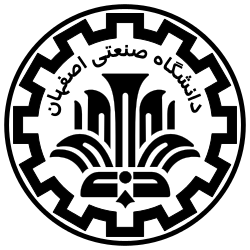
\includegraphics[width=.2\textwidth]{iut}\\
شبکه\ های عصبی مصنوعی\\تکلیف سوم\\
روابط انتشار-به-عقب برای شبکه\ های کانولوشنی
}
\author{داریوش حسن\ پور آده}
\date{۹۳۰۸۱۶۴}
\maketitle
اگر نورون\ های ورودی به صورت یک مربع$N \times N$ در نظر بگیریم و همچنین هریک از نورون\ های کانولوشن به $m \times m$ عدد نورون\ های ورودی متصل باشند، اندازه\ ی لایه\ ی کانولشن برابر خواهد بود با مربعی با تعداد نورون
$(N - m + 1) \times (N - m + 1)$
خروجی نورون\ های لایه\ ی کانولشن را به صورت
\ref{eq:conv_output}
می\ باشد.
\begin{align}
x_{ji}^l &= b + \sum_{l = 0}^{m - 1}\sum_{m = 0}^{m - 1}w_{l,m}\cdot a_{j+l,k+m}\\
y_{ji}^l &= \sigma(x_{ji}^l)\label{eq:conv_output}
\end{align}
در لایه\ ی \lr{Max-Pooling} کار خاصی که نیاز به یادگیری داشته باشد انجام نمی\ دهیم(به این معنی که وزنی بین لایه\ ی کانولوشن و لایه\ ی \lr{Max-Pooling} وجود ندارد) زیرا که فقط خروجی یک دسته\ ی $k \times k$ از لایه\ ی کانولشن را می\ گیرد و حداکثر مقدار آن\ ها را برمی\ گرداند. در نتیجه فقط نیاز داریم که برای وزن\ ها متصل به لایه\ ی خروجی از لایه\ ی \lr{Max-Pooling} و وزن\ های متصل به لایه\ ی کانولوشن از لایه\ ی ورودی را بروز رسانی کنیم.\بند
فرمول\ های انتشار-به-عقب و بروز رسانی وزن\ های متصل به لایه\ ی خروجی از لایه\ ی \lr{Max-Pooling} همانند سابق می\ باشد و تغییری نکرده\ اند. بدین صورت که اگر تابع هزینه\ ی \lr{C} را داشته باشیم روابط
\ref{eq:mp_delta} تا \ref{eq:mp_partial}
را خواهیم داشت. برای محاسبه\ ی انتشار-به-عقب برای وزن\ هایی که از لایه\ ی ورودی به لایه\ ی کانولوشن می\ آیند را با توجه به اینکه از تکنیک وزن\ های مشترک استفاده می\ کنیم باید به ازای هر وزن مقدار
$\p{C}{w_{l,m}}$
 از آنجایی که در لایه\ ی کانولوشن
$(N - m + 1) \times (N - m + 1)$
نورون دارد باید با استفاده از مشتق زنجیره\ ای میزان سهم گرادیانی هر وزن در خطای آن لایه را بدست بیاوریم، که در معادله\ ی
\ref{eq:p_c_w}
آورده شده است.\بند
\begin{align}
\delta^l &=   ((w^{l+1})^T\delta^{l+1}) \odot \sigma^\prime(z^l)\label{eq:mp_delta}\\
\p{C}{b_j^l} &= \delta_j^l\\
\p{C}{w_{jk}^l} &= a_k^{l - 1}\delta_j^l\label{eq:mp_partial}\\\\
{\partial C \over \partial w_{l,m}} 
&= \sum_{i = 0}^{N - m}\sum_{j = 0}^{N - m} \p{C}{x_{ij}^l}\cdot\p{x_{ij}^l}{w_{l,m}}\nonumber\\
&\teq{eq.\ref{eq:conv_output}} \sum_{i = 0}^{N - m}\sum_{j = 0}^{N - m} \p{C}{x_{ij}^l}\cdot a_{i+l,j+m}^{l-1}\label{eq:p_c_w}
\end{align}
علت اینکه در
\ref{eq:p_c_w}
از جمع استفاده شده است بخاطر این است که در لایه\ ی کانولوشن از تکنیک وزن\ های مشترک\زیرنویس{\lr{Weight Sharing}} استفاده شده است. حال برای اینکه مقادیر گرادین را حساب کنیم باید مقادیر
$\delta_{i}^l = \p{C}{x_{ij}^l}$
را به بدست بیاوریم(\کادربی{رابطه\ ی} \ref{eq:final_conv_bp1}).
همچنین برای بروز رسانی وزن\ ها در لایه\ ی کانولشن باید خطا را به لایه\ ی عقبی انتشار دهیم که \کادربی{رابطه\ ی}
\ref{eq:final_conv_bp2}
خطای مرتبط به لایه\ ی پیشین را به ما می\ دهد را خواهیم داشت.
\begin{align}
\p{C}{x_{ij}^l} &= \p{C}{a_{ij}^l}\cdot\p{a_{ij}^l}{x_{ij}^l} = \p{C}{a_{ij}^l}\sigma^\prime(x_{ij}^l)\label{eq:final_conv_bp1}\\
\p{C}{a_{ij}^{l-1}} &= \sum_{i = 0}^{N - m}\sum_{j = 0}^{N - m} \p{C}{x_{(i - l),(j - m)}^l}\cdot\p{x_{(i - l),(j - m)}^l}{a_{ij}^{l-1}}\nonumber\\
&\teq{eq.\ref{eq:conv_output}} \sum_{i = 0}^{N - m}\sum_{j = 0}^{N - m} \p{C}{x_{(i - l),(j - m)}^l}\cdot w_{l,m}\label{eq:final_conv_bp2}
\end{align}
در نهایت وزن\ ها را مطابق معمول بروز رسانی خواهیم کرد.
\begin{equation}
w_{ij}^l = w_{ij}^l - \alpha\p{C}{w_{ij}^l}
\end{equation}
\end{document}
